\begin{tikzpicture}
\begin{visibleenv}<2->
\node (pic) {
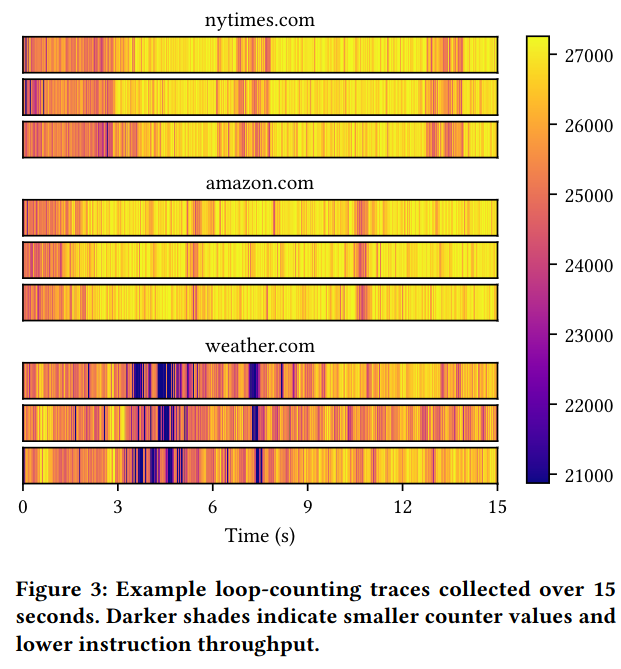
\includegraphics[height=0.6\mypaperheight]{../spectre/website-sigs-fig}
};
\node[anchor=north west,align=left] at (pic.north east) {
turns out, other webpages \\
create distinct ``signatures'' \\
\fontsize{8}{9}\selectfont\parbox{10cm}{Figure from Cook et al, ``There’s Always a Bigger Fish:
Clarifying Analysis of a Machine-Learning-Assisted Side-Channel Attack'' (ISCA '22)}
};
\end{visibleenv}
\end{tikzpicture}